\section{Control Flow Graph}\label{control_flow_graph}
If one wants to analyse a program and the analysis is flow sensitive one can use a Control Flow Graph(CFG) to track the flow of the program.
An analysis flow sensitive means that it is significant in which order pieces of the program are executed.
A CFG is simply just another representation of the program source.
It is a directed graph where a node is a specific place in the program and edges represent the possible options to which the program can execute to.
A CFG always consists of one entry node and one exit node, called \textit{entry} and \textit{exit}.
Given a node \textit{n} the set of predecessor nodes are denoted \textit{pred(n)} and the set of successors are denoted \textit{succ(n)}.

\paragraph{Python control flow graphs}
Control flow graphs for simple Python statements, such as an assignment, have an entry node, a node containing the assignment and an exit node.
The control flow graph of the sequence of two statements $S_1$ and $S_2$ are constructed by deleting the exit node of $S_1$ and the entry node of $S_2$ and \emph{gluing} the two resulting graphs together.
This process is depicted on \cref{cfg_sequence}.

\begin{figure}
  \begin{subfigure}[b]{0.49\textwidth}
    \center
    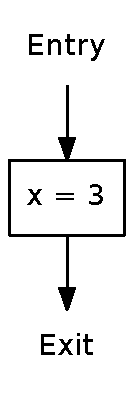
\includegraphics[scale=0.5]{figures/simple.pdf}
    \caption{A single statement}
  \end{subfigure}
  ~
  \begin{subfigure}[b]{0.49\textwidth}
    \center
    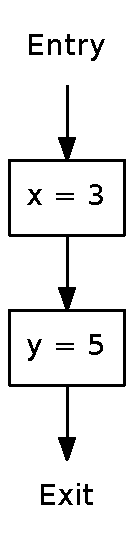
\includegraphics[scale=0.5]{figures/sequence.pdf}
    \caption{A sequence of two statements}
  \end{subfigure}
  \caption{Construction of a control flow graph for two sequential statements}
  \label{cfg_sequence}
\end{figure}

The control flow graphs of  control flow structures in the Python programming language was presented in the figures provided in \cref{python:control_structures}.

\textbf{Note} that the \textit{else} clause is not represented as a independent node, the false branch is represented in the same way as the true branch in a ``if-else'' structure.
\todo{synes maske det skal flyttes til eksemplet, men det kommer an pa hvordan tekster i python eksemplet bliver}

The control flow graph for a complete program is produced by systematically combining the building blocks.
An example of a small program can be seen on \cref{cfg_small_program}

\begin{figure}
  \center
  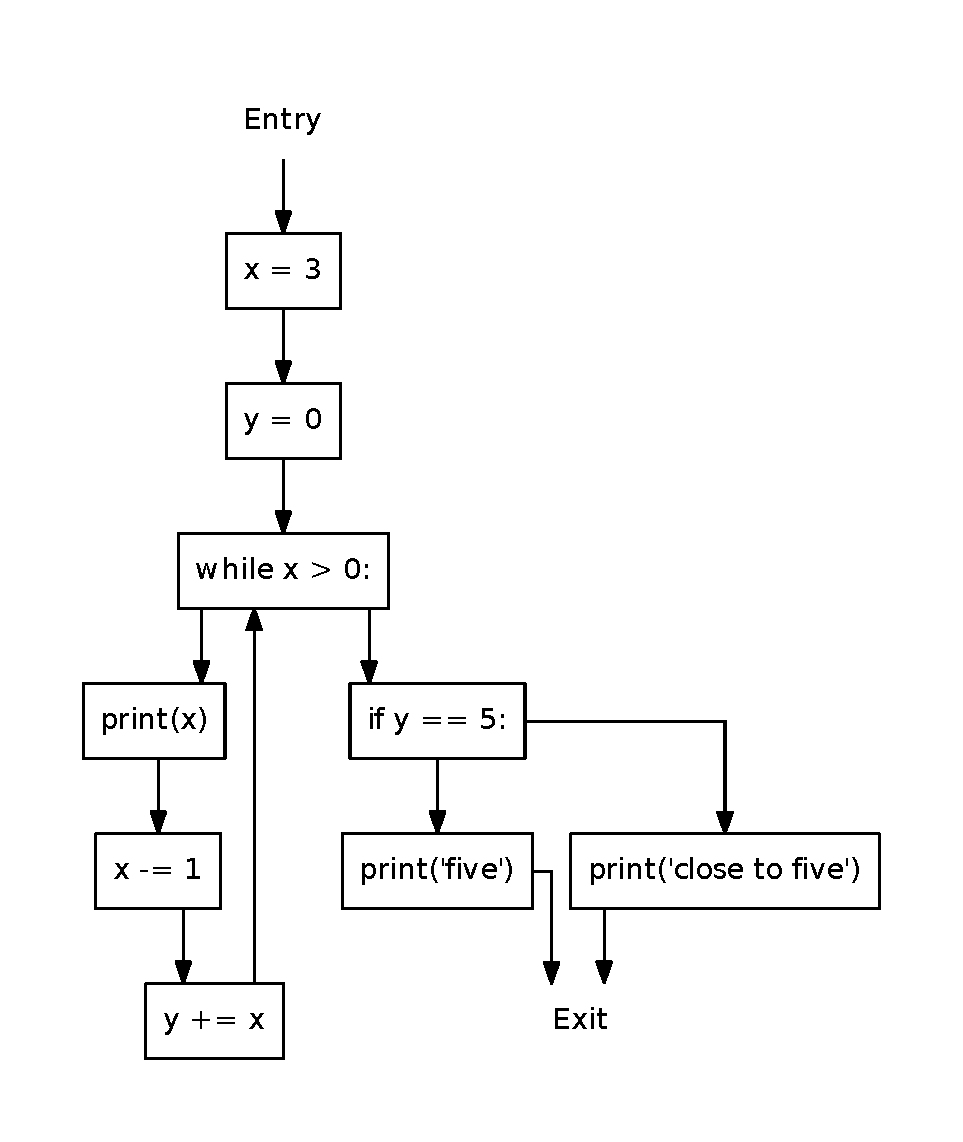
\includegraphics[width=0.5\textwidth]{figures/small_program.pdf}
  \caption{The control flow graph of a small Python program}
  \label{cfg_small_program}
\end{figure}
